\chapter{Návrh}\label{chap:design}

V této kapitole se bude zabývat návrhem úprav a rozšíření původní testovací knihovny


\section{Souhrn požadavků}

K tomu abych mohl správně navrhnout úpravy v testovací knihovně, tak je dobré připomenout, co se od nové knihovny požaduje a proč. Knihovna by ve své nové podobě měla umět spouštět virtualizovaná zařízení a dle konfigurace vytvářet požadované topologie. Hlavní motivací je zvýšení flexibility knihovny, zvýšení možností využití a minimalizovaní zásahu do kódu testovaného zařízení, což vše vede ke snížení nákladů a úsilí na testování.  

Tyto kroky směřují k snížení závislosti na reálném hardwaru, na kterém daný produkt následně poběží. Hardware a primárně jeho architektura ve spoustě případů hraje důležitou roli. Jsou ovšem komponenty, jejichž chování je stejné, ať už poběží na jakémkoliv stroji. Jejich logika si nijak nemění. Přesunutím testů těchto komponent do virtualizovaného prostředí rozšíří možnosti, jak tyto komponenty testovat. Zároveň je možné mít mnohem více testovacích scénářů na různých topologiích. Je ale samozřejmé, že testy na reálném hardwaru budou vždy potřeba a nelze se této závislosti nijak zbavit.


\section{Návrh architektury}

Jednu z možných architekturu stávající testovací knihovny je možné vidět na obrázku \ref{fig:bp_devicemodel}. Jak lze vidět, testovací knihovna požadovala existenci alespoň jednoho fyzického zařízení, tedy reálného zařízení běžícího mimo zařízení, na kterém byla spouštěna testovací knihovna. 
Toto byla velice omezující podmínka, díky které nebylo možné virtualizovat samotné testované zařízení.

Představu nové architektury je možné vidět na obrázku \ref{fig:architecture}. Jak je na obrázku vidět, vše se již odehrává na tzv. agentovy, což je ve finále jakékoliv zařízení s potřebným softwarem pro virtualizaci. Všechna zařízení jsou přesunuta do virtualizovaného prostředí, které bude orchestrováno za pomoci softwaru Docker. 

Na obrázku lze vidět tři druhy zařízení, která jsou barevně oddělená. Zeleně označeným zařízením je původní \textit{testovací služba}. Ta řídí testovací běh a vyhodnocuje výsledky testů. Testovací služba běží přímo v operačním systému agenta, tedy bez žádné virtualizace. Uvnitř modře označeného virtualizovaného prostředí lze následně vidět jednu z možných simulovaných topologií, v tomto případě topologii hvězdy. 

Každý objekt uvnitř virtualizovaného prostředí představuje právě jedno zařízení, které je kontejnerizováno. \textit{Testované zařízení} představuje vyvíjený produkt, který chceme testovat. Ostatní oranžová zařízení představují \textit{testovací partnery} potřebné k testování. Rozdílem od stávající knihovny je, že ne všichni testovací partneři musí být k testovací službě připojeni. Na obrázku lze vidět, že v tomto případě pouze testovací partner 1 a 4 jsou připojeni k testovací službě. Je zde ale předpoklad, že alespoň jedno zařízení musí být k testovací službě připojeno.

Novým typem zařízení je červeně označený \textit{odposlouchávač komunikace}. Toto zařízení jak už z názvu vyplívá bude zaznamenávat komunikaci na právě jednom spojení dvou zařízení. Zároveň bude připojeno k testovací službě, což znamená že komunikace bude zaznamenávána pouze v průběhu testu a pro každý test bude vytvořen separátní záznam.

\begin{figure}[htbp]
    \centering 
    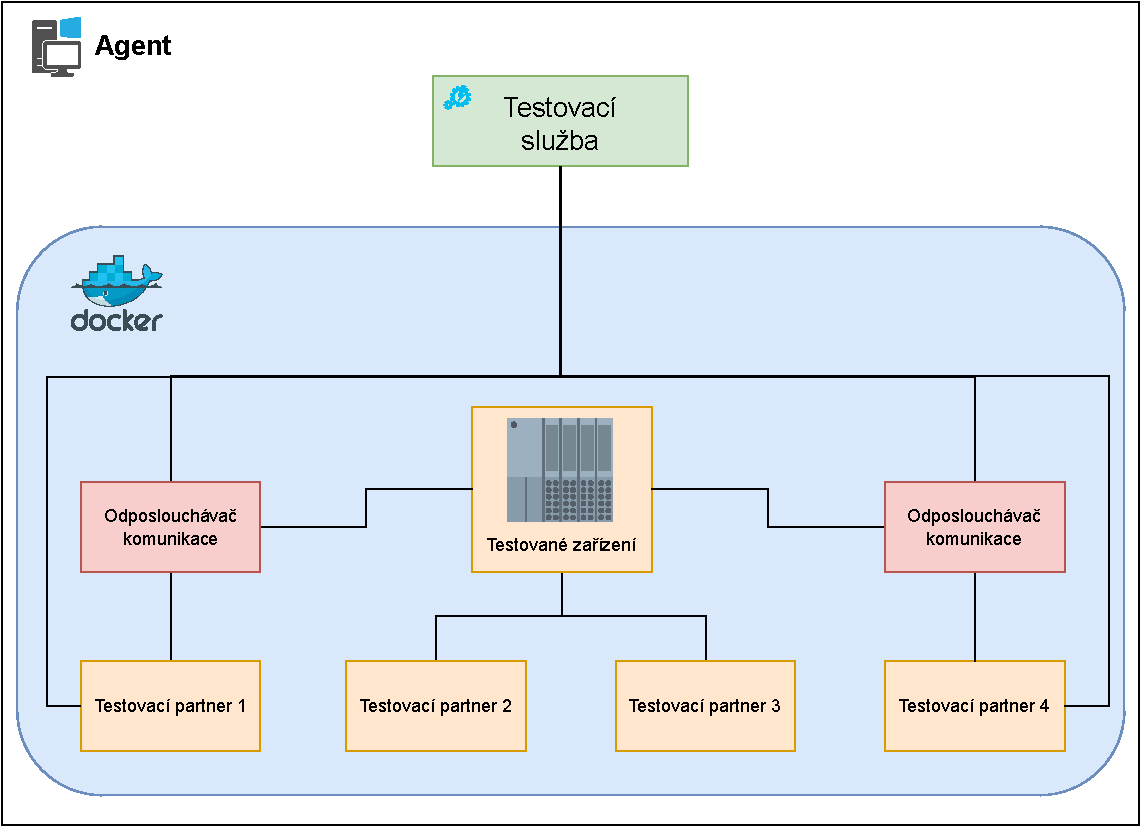
\includegraphics[width=\textwidth]{assets/img/architecture.pdf}
    \caption{Ukázka jedné z možných architektur nové testovací knihovny}
    \label{fig:architecture}
\end{figure}


\section{Orchestrace virtualizovaného prostředí}\label{sec:design_virt}

Důležitou součástí testovací knihovny bude implementace orchestrace virtualizovaného prostředí. To znamená, že testovací služba bude schopna vytvářet jednotlivá virtuální zařízení, které následně automaticky propojí dle požadované topologie a po konci testování daná zařízení ukončí. 

Knihovna bude obsahovat tři správce

\begin{enumerate}
    \item Správce kontejnerů, tedy zařízení
    \item Správce sítě
    \item Správce virtualizovaného prostředí
\end{enumerate}

Veškerá orchestrace bude procházet přes tyto správce. Správce virtualizovaného prostředí bude obsahovat oba předem zmíněné správce. Tyto budou mít na starost existenci daných zdrojů, dle názvu.

Virtualizované prostředí bude definované za pomoci konfiguračního souboru dle formátu YAML. Hlavní důvod proč využít YAML, místo původního formátu JSON, kterým bylo definováno nastavení testovací knihovny, je co nejbližší přiblížení se aktuálním konvencím v kontextu k Docker compose. Konfigurace bude tedy co nejvíce napodobovat jeho konfigurační soubor. 

První položkou v konfiguračním souboru bude položka \inlinecode{service}. Ta bude obsahovat pouze položku \inlinecode{connections}, která bude obsahovat počet zařízení, která se připojí k testovací službě. Toto číslo musí být větší než 0, jelikož testovací knihovna bude alespoň jedno zařízení vyžadovat.

Další položkou bude položka \inlinecode{containers}. Ta bude obsahovat informace o všech zařízeních, která v daném virtualizovaném prostředí budou. Klíčem každé položky uvnitř této sekce bude název zařízení, které bude fungovat pro referenci daného zařízení. Pro každé zařízení následně půjde definovat tato nastavení: 

\begin{description}
    \item[build] Definice zařízení, buď za pomoci obrazu (image) nebo cestou k docker souboru (Dockerfile). Toto bude označeno klíčem \inlinecode{image} a \inlinecode{dockerfile}, následovanou požadovanou hodnotou.
    \item[type] Typ zařízení, které bude vytvořeno. \customtodo{upřesnit}
    \item[cap\_add] Seznam \uv{schopností}, v tomto kontextu práv, které bude daný účet na kontejneru mít. Ty budou přidány ke právům, které v základu docker dává účtu vytvořenému v kontejneru. 
    \item[commands] Seznam příkazů, které budou spuštěny v kontejneru.
    \item[environment] Seznam proměnných, která budou v kontejneru nastaveny. Klíč bude název proměnné a jeho hodnota bude hodnotou proměnné
    \item[ports] Seznam mapování portů z kontejneru do prostředí hostitelského zařízení. Každý záznam obsahuje dva porty oddělené dvojtečkou, kdy první je port hostitelského zařízení a druhý je port kontejnerizovaného zařízení.
    \item[privileged] Boolean hodnota, zdali účet na kontejneru bude mít administrátorské práva.
    \item[logging] Boolean hodnota, která značí zdali je komunikace mezi tímto zařízením odposlouchávána. Tedy pokud je hodnota \inlinecode{true}, tak poté knihovna zařídí zaznamenávání všech spojů tohoto zařízení
    \item[tty] Boolean hodnota, která v původním docker compose značí připojení pseudo-terminálu ke kontejneru, který má za následek to, že kontejner po dokončení definovaných příkazů zůstane běžet. V kontextu knihovny bude znamenat to, že kontejner zůstane po dokončení všech příkazů definovaných v \inlinecode{commands} běžet. 
\end{description}

V neposlední řadě konfigurační soubor bude obsahovat položku \inlinecode{links}. Ta bude definovat jednotlivá propojení mezi zařízeními, tedy celkovou topologii. V tomto seznamu bude každá položka obsahovat názvy dvou zařízení oddělené dvojtečkou a pro každý záznam bude vytvořeno propojení mezi danými zařízeními.

Povinnou součástí konfiguračního souboru bude celá sekce \inlinecode{service}, sekce \inlinecode{containers}, kde musí být definována nejméně jedno zařízení, která musí obsahovat alespoň kolonky \inlinecode{build} a \inlinecode{type}, a sekce \inlinecode{links}. Ostatní budou nepovinné. Při existenci pouze jednoho zařízení může být testovací knihovna využita pro unit testy. 

Testovací knihovna bude kontrolovat, zdali testované prostředí bylo vytvořeno. Pokud ne, nezapočne testování. Zároveň bude kontrolovat zda všechna zařízení byla úspěšně spuštěna. Po konci testování testovací knihovna všechna zařízení ukončí, a vymaže všechny jím definované sítě, kontejnery atd.

Pro pohodlnost testovací knihovna bude také podporovat více různých topologií v rámci jednoho testovacího projektu. Při každé inicializaci virtualizovaného prostředí testovací služba porovná danou konfiguraci s aktuální konfigurací. Pokud budou konfigurace totožné, testovací služba ponechává prostředí nepozměněné, v opačném případě vyčistí virtualizované prostor, do kterého následně vloží nová zařízení a jejich nastavení.  


\section{Komunikace}

Komunikaci v rámci testovací knihovny lze rozdělit do dvou kategorií:

\begin{enumerate}
    \item komunikace mezi zařízeními,
    \item komunikace s testovací službou.
\end{enumerate}

Propojení mezi jednotlivými zařízeními bude zprostředkováno testovací knihovnou, respektive všechny zařízení budou propojena dle dané konfigurace, ale nebude nijak kontrolováno, pouze dle požadavku může být komunikace odposlouchávána a ukládaná. 

Komunikace s testovací službou bude probíhat za stejných podmínek, jako tomu je doposud. Testovací knihovna přesně definuje strukturu zpráv. Každá zpráva obsahuje v prvních dvou bajtech typ zprávy, v dalších dvou bajtech délku dat zprávy a případná data zprávy, jejichž délka je uložena v délce dat zprávy. Každá zpráva tedy musí mít minimálně 4 bajty. 

Možnou komunikaci mezi testovací službou a účastníky testu, tedy zařízeními uvnitř virtualizovaného prostředí, můžeme vidět na sekvenčním diagramu z mé bakalářské práce\cite{bakalarka}, který je na obrázku \ref{fig:seqdiag}. Na něm lze vidět, jak by probíhala komunikace při běhu o jednom testu. Jak jsem již ale zmínil dříve, nově ne všechna zařízení musí komunikovat s testovací službou. 

\begin{figure}[htbp]
    \centering 
    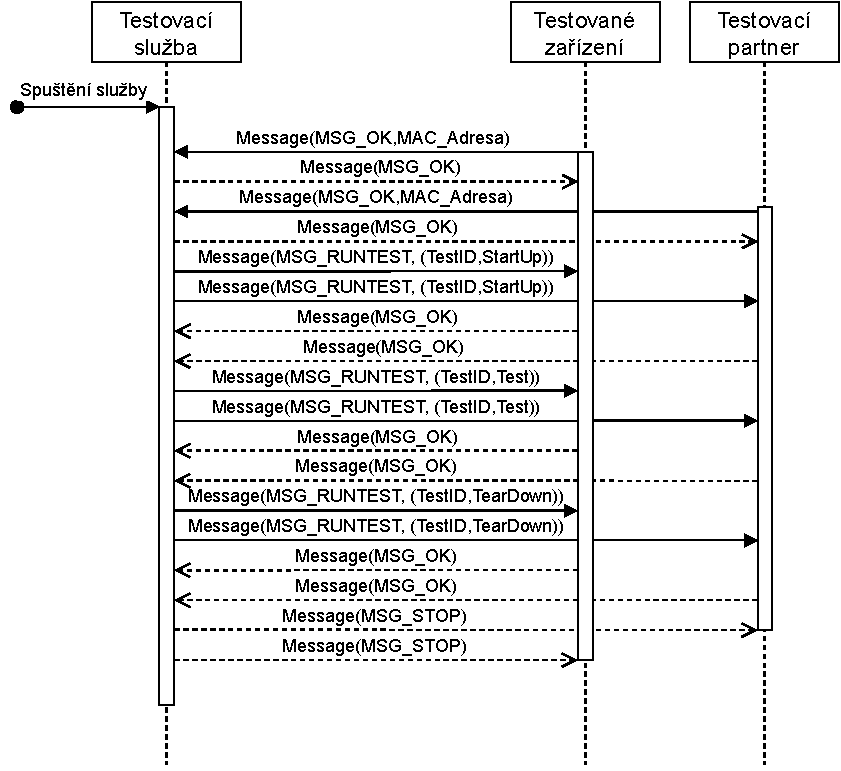
\includegraphics[width=\textwidth]{assets/img/bp_assets/sequencediagram.pdf}
    \caption{Sekvenční diagram ukázky komunikace mezi účastníky testování}
    \source{Převzato z \cite{bakalarka}}
    \label{fig:seqdiag}
\end{figure}

\section{Testovací služba}

Jádrem testovacího běhu zůstane testovací služba, která musí komunikovat a tím ovládat alespoň jedno zařízení. Ve stávající implementaci byla na počátku testování vytvořena jedna instance testovací služby, která existovala po celou dobu testování. Nově bude životnost testovací služba navázána na dané virtualizované prostředí. Tedy, testovací služba vznikne až po úspěšném vytvoření virtualizovaného prostředí. Při změně virtualizovaného prostředí bude testovací služba ukončena a po vytvoření nového prostředí spuštěna nová instance.

Fungování testovací služby lze vidět na novém diagramu aktivit testovací služby na obrázku \ref{fig:activitydiagramservice}, na kterém jsou označeny i změny oproti původnímu diagramu aktivit testovací služby.

\begin{figure}[htbp]
    \centering 
    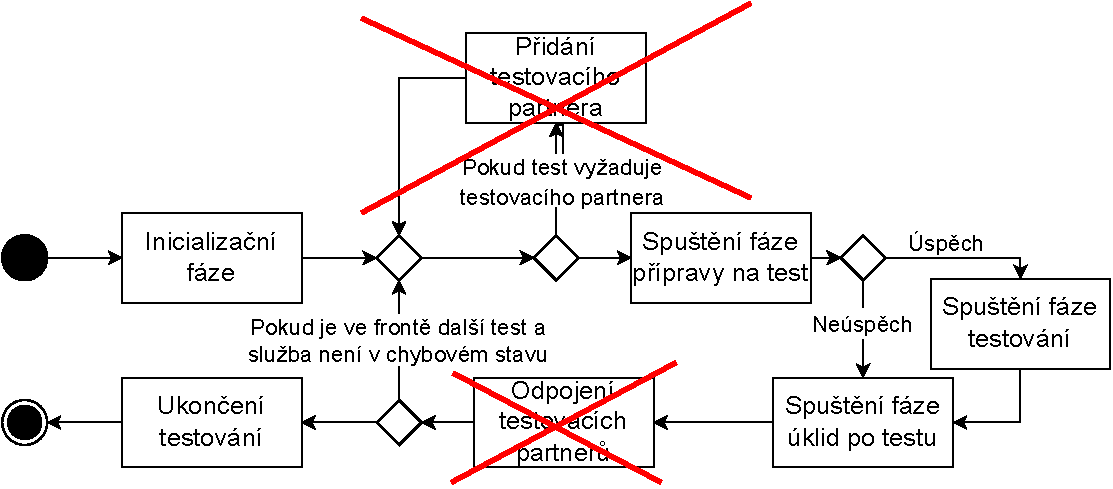
\includegraphics[width=\textwidth]{assets/img/activitydiagramservicechange.pdf}
    \caption{Nový diagram aktivit testovací služby}
    \source{Vytvořeno dle předlohy z \cite{bakalarka}}
    \label{fig:activitydiagramservice}
\end{figure}

Po sestavení virtualizovaného prostředí testovací služba započne inicializační fázi, ve které se všechna zařízení ovládaná testovací službou připojí k testovací službě. Tedy mimo přímých účastníků testu se v této fázi připojí i všichni odposlouchávači komunikace, pokud nějací existují. 

Testovací služba sama o sobě nemá ponětí o tom, které testy budou spuštěny a které ne, ale pouze zpracovává požadavky, které na ni přichází. Tedy po obdržení požadavku na spuštění testu testovací služba spouští všechny fáze testu. Při ukončení testovací služba odesílá všem připojeným účastníkům zprávu o ukončení testování, čímž mohou být připojená zařízení taktéž ukončena. O úspěšné ukončení se ovšem stará integrace virtualizovaného prostředí.

\section{Testování}

Nová testovací knihovna zachová proces testování a podobu jednotlivých testu ve stejné podobě jako tomu bylo doposud. K tomu aby bylo možné testovat za použití testovací knihovny, tak je potřeba implementovat rozhraní pro testované zařízení, které definuje potřebné funkce ke komunikaci s testovací službou. 

Definované rozhraní je ale v rámci terminologie nyní lepší nazvat jako rozhraní pro účastníka testu, jelikož rozhraní může využít jakékoliv zařízení, které je potřeba synchronizovat s testovací službou. I v aktuální implementaci testovací partneři obsahovali implementaci tohoto rozhrání a jejich běh byl identický. 

Pro připomenutí, rozhraní pro test následně definuje tři fáze testu, které jsou:

\begin{enumerate}
    \item Příprava na testování -- definování potřebných struktur, inicializace.
    \item Testování -- provedení samotného testu.
    \item Úklid po testu -- uvolnění využitých zdrojů a uvedení zařízení do původního stavu.
\end{enumerate}

Běh účastníka testu, který je připojen k testovací službě, můžeme vidět na diagramu aktivit na obrázku \ref{fig:act_diag_device}. Jeho aktivity zůstanou identické. Změna nastává v definovaných synchronizačních bodech, které jsou na obrázku označeny modře. 

Testovací služba obdrží informace o dokončení každé fáze testu pouze od těch účastníků, co jsou k ní připojený. Tedy, pokud je potřeba synchronizovat nějaké zařízení, které není připojeno k testovací službě, tak potom by toto byl úkol jednoho z testovacích partnerů, který k testovací službě připojen je. Zároveň zde existuje možnost vytvořit testovacího partnera, který pouze kontrolovat správnost daného zařízení. 

\begin{figure}
    \centering 
    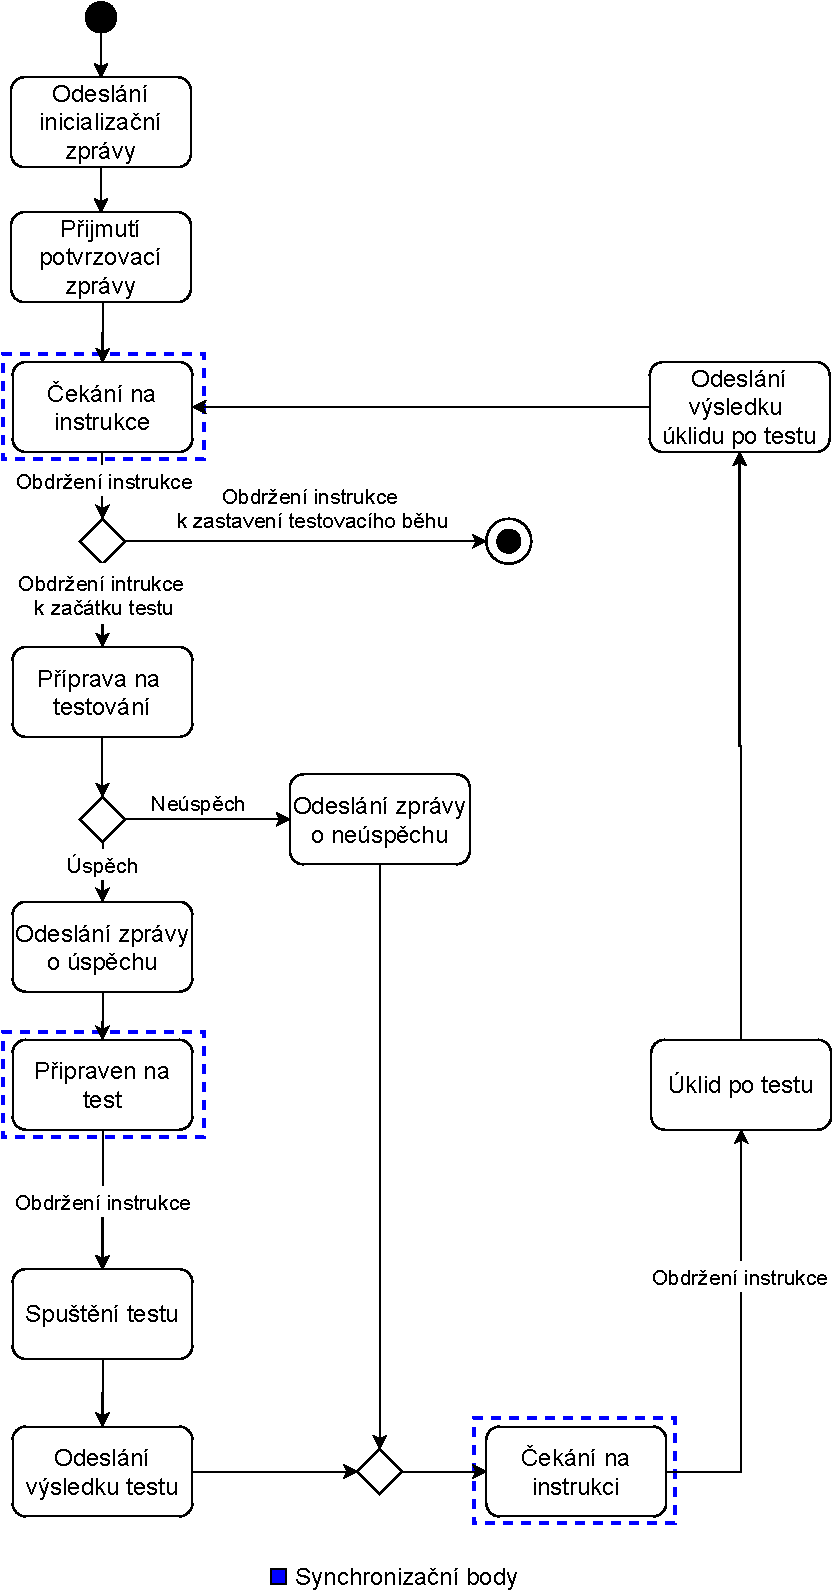
\includegraphics[height=0.98\textheight]{assets/img/bp_assets/activitydiagramdevice.pdf}
    \caption{Diagram aktivit účastníka testu}
    \label{fig:act_diag_device}
\end{figure}



